\section{Common-witness geometry and interval tools}
\label{sec:geometry}

Using the notation of Definition~\ref{def:normalized-queries},
we prove the structural facts shared by both algorithms.
Algorithm~\ref{alg:hull-data} records their common preprocessing.
For a flat state, Helly's theorem gives a common majority witness.
Relative to this witness, each query cap is covered by at most two
adjacent hull caps, so every hypothesis's positive hull answers form
one circular interval. The interval tools below use this structure to
discover patterns and decode their endpoints.

\begin{proofstrategy}
\begin{enumerate}
\item Flatness makes every three majority half-planes intersect;
Helly's theorem gives a common strict witness.
\item Radial projection onto the normalized query hull supplies
adjacent supports; a half-plane reads one circular positive interval.
\item Interval covers discover a positive vertex, after which a
query-free cut turns supplied hull tests into endpoint comparisons.
\end{enumerate}
\end{proofstrategy}

\begin{symboltable}
$p,\ x_h,\ u_i$ & Strict common witness, translated hypothesis vector $h-p$, and normalized vector for supplied line $\ell_i$.\\
$C_i,\ R_h$ & Original-plane cap opposite $p$ for query $i$, and the dual set of normalized queries positive on $h$.\\
$K,\ V$ & Convex hull of the normalized query vectors together with $0$, and its nonzero vertices in cyclic order.\\
$J_i,\ \alpha_{iv}$ & At most two adjacent support vertices for $u_i$ and their nonnegative coefficients, whose sum is at most one.\\
$\sigma(h),\ \Pi$ & Hull-test bit pattern of $h$ and the partition into equal-pattern classes.\\
$A_0,\ b(S)$ & All-zero pattern class (empty if absent) and, with priors, the mass outside that class.\\
$g_A$ & First positive test position for a nonzero pattern class $A$ in a discovery schedule.\\
\end{symboltable}

\subsection{A common majority witness}

The majority answers must describe one coherent route before we can
compare our discovery schedule with an optimal tree. A common witness
provides that route even when no hypothesis has all majority answers.

\begin{lemma}[Common witness]\label{lem:helly}
In either kind of flat state, a point $p$ strictly inside every
majority half-plane can be computed in polynomial time.
\end{lemma}
\begin{proof}
Flatness forces every three majority sides to intersect.
Claim~\ref{clm:majority-triples} and Theorem~\ref{thm:helly}
therefore give a common strict point. Claim~\ref{clm:rational-witness}
then finds a rational one by a positive-margin linear program.
\end{proof}

\subsection{Adjacent supports and circular patterns}

The witness lets us express every query relative to the same origin.
The next lemma identifies the two properties that make this useful:
each original cap is covered by adjacent hull caps, and each target
sees those hull tests as one interval.

\begin{lemma}[Hull support and pattern structure]\label{lem:hull-structure}
The support blocks of Definition~\ref{def:normalized-queries} can
be chosen with at most two real hull vertices, adjacent when there
are two. For every query,
\begin{equation}\label{eq:hull-cap-cover}
 C_i\cap S\ \subseteq\ \bigcup_{v\in J_i}(C_v\cap S).
\end{equation}
Negative support bits force the query's witness-side answer.
The positive vertices of every hypothesis form a circular interval,
$|A_0|\le1$, and every nonzero pattern class lies in a positive hull cap.
\end{lemma}
\begin{proof}
Claim~\ref{clm:radial-supports} projects each query vector radially
to a hull edge, and Claim~\ref{clm:negative-supports} shows that
its adjacent endpoints cover that query's cap.
Claim~\ref{clm:circular-patterns} then proves the interval structure
and uses separability to bound the all-zero class.
\end{proof}

The routine first finds a point that satisfies every oriented majority
inequality, then uses that common witness to normalize the supplied
query normals into a planar hull. The supports $J_i$ retain the
queries represented by each hull direction; grouping hypotheses by
their resulting bit vectors gives the full-pattern classes needed by
the recursive algorithms. Lemmas~\ref{lem:helly} and
\ref{lem:hull-structure} justify the witness and support invariant.

\begin{algorithm}[H]
\caption{\HullData: a flat state's witness, supports, and patterns}
\label{alg:hull-data}
\KwIn{Flat state $S$ and its count or mass measure; supplied lines.}
\KwOut{Strict witness $p$, full hull $K$, real vertices $V$, supports $J_i$, partition $\Pi$.}
Orient every majority inequality as $a_i\cdot p-b_i>0$\;
Maximize $t$ subject to $a_i\cdot p-b_i\ge t$ and $0\le t\le1$;
retain a solution with $t>0$\;
Compute $u_i=-a_{\ell_i}/f_{\ell_i}(p)$ and
$K=\operatorname{conv}(\{0\}\cup\{u_i\})$\;
Keep one supplied representative of each real hull vertex in cyclic order\;
\ForEach{$u_i$}{
Extend its ray from $0$ to the last point $y$ in $K$\;
Express $y$ on its boundary edge and scale the coefficients by
$\|u_i\|/\|y\|$; omit the origin and zero coefficients to form $J_i$\;
}
Compute all bits $\mathbf1[v\cdot(h-p)>1]$ and group equal rows into $\Pi$\;
\KwRet $(p,K,V,(J_i),\Pi)$, retaining the origin's boundary position\;
\end{algorithm}

When the normalized hull has dimension at most one, its segment
endpoints provide the supports directly.


Figure~\ref{fig:support-and-interval} separates the two geometric
roles: panel (a) shows how adjacent hull vertices support an original
query vector, while panel (b) records only the cyclic order of the
hull tests seen positively by one hypothesis.

\begin{figure}[tbp]
\centering
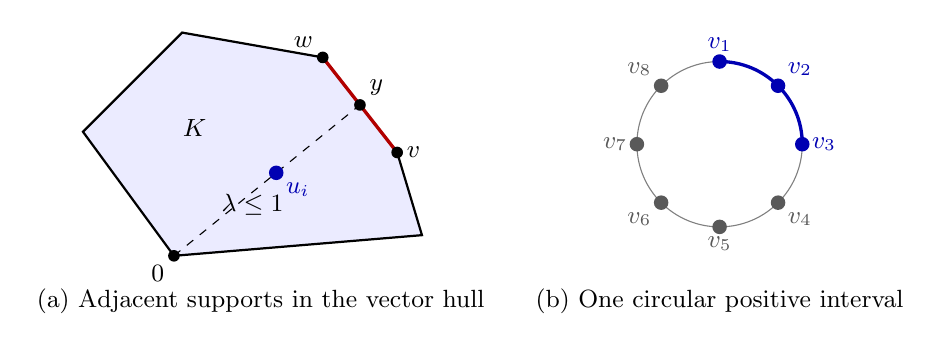
\begin{tikzpicture}[scale=1.05,every node/.style={font=\small}]
  % Query vectors and their adjacent hull supports.
  \fill[blue!8]
    (0,0)--(3,0.25)--(2.7,1.25)--(1.8,2.4)--(0.1,2.7)
    --(-1.1,1.5)--cycle;
  \draw[thick]
    (0,0)--(3,0.25)--(2.7,1.25)--(1.8,2.4)--(0.1,2.7)
    --(-1.1,1.5)--cycle;
  \draw[very thick,red!70!black] (2.7,1.25)--(1.8,2.4);
  \draw[dashed] (0,0)--(2.25,1.825);
  \fill (0,0) circle (2pt) node[below left] {$0$};
  \fill (2.7,1.25) circle (2pt) node[right] {$v$};
  \fill (1.8,2.4) circle (2pt) node[above left] {$w$};
  \fill (2.25,1.825) circle (2pt) node[above right] {$y$};
  \fill[blue!70!black] (1.2375,1.00375) circle (2.5pt)
    node[below right] {$u_i$};
  \node at (0.25,1.55) {$K$};
  \node at (0.95,0.62) {$\lambda\le1$};
  \node[align=center] at (1.05,-0.55)
    {(a) Adjacent supports in the vector hull};

  % A schematic cyclic order; blue vertices form one interval.
  \draw[gray] (6.6,1.35) circle (1);
  \draw[very thick,blue!70!black]
    (6.6,2.35) arc[start angle=90,end angle=0,radius=1];
  \fill[blue!70!black] (6.6,2.35) circle (2.5pt)
    node[above] {$v_1$};
  \fill[blue!70!black] (7.307,2.057) circle (2.5pt)
    node[above right] {$v_2$};
  \fill[blue!70!black] (7.6,1.35) circle (2.5pt)
    node[right] {$v_3$};
  \fill[gray!70!black] (7.307,0.643) circle (2.5pt)
    node[below right] {$v_4$};
  \fill[gray!70!black] (6.6,0.35) circle (2.5pt)
    node[below] {$v_5$};
  \fill[gray!70!black] (5.893,0.643) circle (2.5pt)
    node[below left] {$v_6$};
  \fill[gray!70!black] (5.6,1.35) circle (2.5pt)
    node[left] {$v_7$};
  \fill[gray!70!black] (5.893,2.057) circle (2.5pt)
    node[above left] {$v_8$};
  \node[align=center] at (6.6,-0.55)
    {(b) One circular positive interval};
\end{tikzpicture}
\caption{The first panel depicts normalized query vectors: $y$ lies
on the edge $vw$ and $u_i=\lambda y$ for
$0<\lambda\le1$. Writing $y=\theta v+(1-\theta)w$ gives
$u_i=\alpha v+\beta w$ with $\alpha+\beta=\lambda\le1$.
Consequently, if both support values on a hypothesis are at most
one, then $u_i\cdot x_h\le1$; equivalently,
$C_i\subseteq C_v\cup C_w$. The second panel shows the cyclic order
only; the positive hull tests of a fixed hypothesis form one
interval in that order.}
\label{fig:support-and-interval}
\end{figure}

\subsection{Interval hitting and discovery length}

A complete discovery route must hit every nonzero pattern. Once these
patterns are intervals, we can compute its smallest possible test set;
this will also provide the final budget in the batch construction.

\begin{lemma}[Minimum interval cover]\label{lem:minimum-interval-cover}
A minimum-cardinality hitting set for ordinary or circular intervals
on a finite candidate order is computable in polynomial time.
An empty demand is infeasible; an empty family needs no candidates.
\end{lemma}
\begin{proof}
On a line, an exchange argument permits choosing the right endpoint
of the earliest-ending demand. On a circle, enumerate one forced
hit and cut there; the remaining problem is linear. The detailed
exchange argument is given below.
\end{proof}

Priority and weight considerations can change the order in which tests
are chosen. We therefore also need a length bound for greedy discovery,
including the extra saving when the comparison cover has adjacent runs.
Here a demand is a nonempty interval of candidate positions, each demand
$I$ has a fixed weight $w(I)>0$, and a candidate's remaining weight is
the sum of $w(I)$ over currently unhit demands containing it. At each
step greedy chooses a candidate of maximum remaining weight; ties may
be resolved arbitrarily. The comparison cover $P$ is any finite set of
positions hitting every initial demand, $k=|P|$, and $c(P)$ counts its
maximal consecutive blocks in the full candidate order. After a greedy
choice, demands hit by that choice are deleted. The claimed bound holds
for every such cover $P$; taking a minimum cover gives the stated
special case.

\begin{lemma}[Greedy cover length with adjacent-run credit]
\label{lem:greedy-cover-length}
Let a nonempty family of positively weighted interval demands
be covered by a candidate set $P$ of size $k$. Let $c(P)$ be the
number of runs of consecutive candidates in $P$, measured in the
entire candidate order. Maximum-remaining-weight greedy finishes
within $k+c(P)-1$ choices, for every tie rule.
In particular, a minimum cover of size $k$ gives the usual bound
$2k-1$. For circular intervals the corresponding bound is $2k$.
\end{lemma}
\noindent
The extra term is the number of runs beyond the first. A scattered
cover may force greedy to spend choices repairing several gaps,
whereas a cover arranged in a few contiguous blocks has fewer such
gaps to repair.
\begin{proofstrategy}
Use the potential $|P|+c(P)$ for the still-active comparison cover.
An extreme choice can replace an extreme point of $P$ without changing
which positive-weight demands it hits. An interior choice partitions
the unhit demands into left and right interval families. The cover
parts on those sides have combined size plus run count at most the
previous potential. Induction pays for the first choice and then for
each nonempty side.
\end{proofstrategy}
\begin{proof}
Induct on the comparison cover size, separating extreme choices from
interior ones. Suppose first that the greedy choice $v$ lies left
of $P$, and let $u=\min P$. Every active interval containing $v$ also
contains $u$: it is covered by some $p\in P$, and the endpoint
inequalities give $v<u\le p$ inside that interval. Thus the hit-demand
set of $v$ is contained in the hit-demand set of $u$. Maximum remaining
weight gives $W(u)\le W(v)$, while containment and nonnegative weights
give $W(v)\le W(u)$. Since each weight is positive, the sets are equal,
so the two hit sets coincide. After querying $v$, every remaining
demand therefore avoids $u$ and is covered by some point of
$P'=P\setminus\{u\}$. The right extreme is symmetric. Since $u$ is an
extreme point, deleting it cannot split a run, so
$|P'|=k-1$ and $c(P')\le c(P)$. If demands remain, induction bounds
their greedy completion by
\[
 |P'|+c(P')-1\le k+c(P)-2.
\]
Including the current query gives at most $k+c(P)-1$ choices. If no
demand remains, the single current query already meets that bound.

Now suppose the greedy choice $v$ is interior. Every unhit interval lies wholly to one
side of $v$. Let $P_-$ and $P_+$ be the comparison points strictly to
its left and right. They cover the corresponding families. If $v\notin
P$, cutting the original order in its gap preserves the total number
of runs, so $c(P_-)+c(P_+)\le c(P)$ and their sizes sum to $k$.
If $v\in P$, the side sizes sum to $k-1$, and deleting $v$ can split
at most one run into two, so $c(P_-)+c(P_+)\le c(P)+1$. In either
case,
\[
 |P_-|+c(P_-)+|P_+|+c(P_+)\le k+c(P).
\]
The induction hypotheses bound the two side schedules by their
respective potentials minus one. Adding the current choice gives at
most $k+c(P)-1$. When only one side remains active, the unused side
has at least one comparison point and hence potential at least two;
this pays for the absent induction term. When neither side remains,
one choice is within the bound because $k\ge2$ in the interior case.
Finally $c(P)\le k$, since each run contains a distinct point of $P$;
therefore $k+c(P)-1\le2k-1$. For circular demands, the first greedy
choice cuts the circle and leaves ordinary intervals; the original
$k$ points still cover those intervals, giving at most $2k-1$ further
choices and the bound $2k$.
\end{proof}

\subsection{Recovering the interval endpoints}
\label{sec:endpoint-geometry}

A positive vertex locates a small cap. We recover the full pattern by
opening the circular order at a safe cut and comparing the interval's
endpoints against the supplied queries.

\begin{lemma}[Query-free endpoint representation]
\label{lem:legal-endpoint-queries}
After one positive hull vertex $v$ is known, a cut computable without
queries represents every compatible positive pattern as an ordinary
interval containing $v$. Supplied hull tests compare its endpoint
coordinates. A cached negative neighbor fixes one endpoint; two
negative neighbors fix the entire pattern.
\end{lemma}
\begin{proofstrategy}
Use a cached negative neighbor as the cut when available. Otherwise
the origin and an opposite hull edge give a cut that no compatible
positive interval can cross. All later comparisons are actual hull
tests, so no new line or anchor query is introduced.
\end{proofstrategy}
\begin{proof}
A cached negative neighbor supplies a cut and pins one endpoint.
Otherwise an opposite hull edge gives a cut without asking a query.
In the resulting linear order, supplied hull tests are endpoint
comparisons. Claims~\ref{clm:cached-endpoint},
\ref{clm:opposite-edge-cut}, and~\ref{clm:supplied-endpoint-comparisons}
establish these steps, including degenerate hulls.
\end{proof}

A positive discovery exit is \emph{pinned} if a neighbor of its
discovered vertex has a cached negative answer. It is
\emph{singly pinned} when exactly one neighbor is known negative,
and \emph{doubly pinned} when both are. Pinning fixes one or both
endpoints, as in Lemma~\ref{lem:legal-endpoint-queries}; it introduces no additional query.

\begin{algorithm}[H]
\caption{\EndpointCode: legal full-pattern recovery}
\label{alg:endpoint-code}
\KwIn{A positive hull vertex $v$, compatible patterns, cached answers;
code mode; optionally fixed continuation heights $h_A$.}
\KwOut{A supplied-query decoder whose leaves are full pattern classes.}
\If{the hull has dimension at most one}{\KwRet the already determined nonzero pattern\;}
\eIf{$v$ has a cached negative neighbor}{
  Cut at that neighbor and orient so $v$ is the first positive vertex\;
}{
  Cut at a boundary origin, or at the opposite edge met by the ray $v0$\;
}
List the realized left and right endpoint pairs in the cut order\;
\eIf{no continuation heights are supplied}{
  Search each unfixed endpoint using Algorithm~\ref{alg:alphabetic-code};
  condition the second search on the first answer\;
}{
  \ForEach{nonempty realized endpoint rectangle $U$, in increasing size}{
    \eIf{$U$ has a single realized class $A$}{$E(U)\gets h_A$\;}{
      $E(U)\gets\min_\ell(1+\max\{E(U\cap\ell^-),E(U\cap\ell^+)\})$,
      over proper supplied endpoint thresholds\;
    }
  }
  Reconstruct the minimizing rectangle splits, retaining full-pattern
  leaves and their recorded continuation heights\;
}
\KwRet the decoder; skip fixed endpoints and cached thresholds\;
\end{algorithm}

The cut turns the cyclic endpoint problem into a linear one, and
Lemma~\ref{lem:legal-endpoint-queries} shows that its thresholds are
supplied queries, so no extra anchor query is needed. If child heights
are provided, the rectangle recurrence compares each legal split by
the height of its endpoint subproblems together with the continuation
at the resulting pattern leaf. This is the complete-exit optimization
of Section~\ref{sec:polynomial-slots}. Its $O(M^4)$ rectangles and
$O(M)$ thresholds give polynomial running time. The routine returns
pattern leaves, after which the recursive algorithm attaches each
stored child once. The values $E(U)$ include the continuation heights
when comparing splits, while each child's query cost is accounted for
inside its attached recursive tree.



\subsection{Proofs of the geometric and interval facts}

The key step is to convert planar caps into executable endpoint
comparisons. Radial projection gives the one-way cover implication
needed by the analysis: every positive original cap is covered by its
support caps. The endpoint cut then follows from the geometry or from
cached answers, so it requires no additional query.

\begin{proof}[Proof of Lemma~\ref{lem:helly}]
There are two distinct tasks: obtain a common strict point from
flatness, then find such a point with controlled rational encoding.
The following claims separate the geometric existence argument from
its algorithmic realization.

\begin{claim}[Three majority half-planes have a common strict point]
\label{clm:majority-triples}
Every subfamily of at most three majority half-planes intersects.
\end{claim}
\begin{proof}
Use the measure defining flatness, either cardinality or probability.
By Definition~\ref{def:balanced}, each minority cap has measure
less than $\delta$ times the measure of $S$. The union bound
therefore makes the union of any three such caps have measure
less than $3\delta$ times that of $S$. Since $3\delta<1$,
that union omits a hypothesis.
That hypothesis belongs strictly to all three majority half-planes,
because no hypothesis lies on a query line. The same argument covers
subfamilies of fewer than three lines. Thus every subfamily of at
most three majority half-planes has nonempty intersection.
Theorem~\ref{thm:helly} implies
that the whole family has nonempty intersection.
\end{proof}

We now turn this strict intersection into the preprocessing algorithm's
witness. A positive-margin linear program finds a rational point with
polynomial encoding length, so the algorithm can compute and store it.

\begin{claim}[A positive margin gives a rational strict witness]
\label{clm:rational-witness}
The common point can be found with polynomial encoding length.
\end{claim}
\begin{proof}
To obtain a strict rational witness, orient each majority inequality
as $a_i\cdot p-b_i>0$ and maximize $t$ subject to
$a_i\cdot p-b_i\ge t$ for every $i$ and $0\le t\le1$.
The strict point obtained from Claim~\ref{clm:majority-triples}
and Theorem~\ref{thm:helly} has a positive value in each of the
finitely many inequalities. Their minimum, capped at one, supplies
a feasible positive $t$.
This is a \emph{linear program}: its objective and constraints
are linear in the unknown coordinates of $p$ and the margin $t$.
Rational linear programming therefore returns a strict witness
with polynomial encoding length~\cite{khachiyan1979}.
\end{proof}
\end{proof}

\begin{proof}[Proof of Lemma~\ref{lem:hull-structure}]
We establish the structure in three steps. First represent each query
by neighboring hull vertices; next prove the cap-cover implication;
finally identify the interval patterns and the unique possible
all-zero target. Each step is used by a different part of the algorithms.

\begin{claim}[Radial boundary projection needs only adjacent supports]
\label{clm:radial-supports}
Each normalized vector has a nonnegative support expression whose
coefficients sum to at most one.
\end{claim}
\begin{proof}
Extend the ray from $0$ through $u_i$ to its last point $y$ in $K$.
Such a point exists because the finite hull is compact and contains
$u_i\ne0$. Write $y=t u_i$ with $t\ge1$, so
$u_i=\lambda y$ for $\lambda=1/t\in(0,1]$.
If $y$ lies on an edge with endpoints $v,w$, write
$y=\theta v+(1-\theta)w$, with $0\le\theta\le1$. Then
\[
 u_i=(\lambda\theta)v+\lambda(1-\theta)w,\qquad
 \lambda\theta+\lambda(1-\theta)=\lambda\le1.
\]
The coefficients are nonnegative. Delete origin endpoints and zero coefficients
to obtain $J_i$. A boundary vertex needs only itself.
In dimension at most one, the last ray point is a segment endpoint,
so the same conclusion holds directly.
\end{proof}

The support expression is useful because it transfers a negative
answer from the hull tests back to the original query. Only this
one-way implication is needed to cover an optimal witness route.

\begin{claim}[Negative support answers force the original answer]
\label{clm:negative-supports}
The hull-cap inclusion \eqref{eq:hull-cap-cover} holds.
\end{claim}
\begin{proof}
If every support has $v\cdot x_h\le1$, the expression from
Claim~\ref{clm:radial-supports} gives
\[
 \begin{aligned}
 u_i\cdot x_h
 &=\sum_{v\in J_i}\alpha_{iv}(v\cdot x_h)\\
 &\le\sum_{v\in J_i}\alpha_{iv}\le1.
 \end{aligned}
\]
The first inequality uses the nonnegative support coefficients;
the second uses their sum bound. Thus a positive original query
must have a positive support, proving
\eqref{eq:hull-cap-cover}. Equality cannot occur at a hypothesis
because it would put it on the original supplied line.
The origin has dot product zero, so its bit is always negative
and it is never queried.
\end{proof}

Having justified cap coverage, we now describe the states produced
by hull tests. Their interval structure enables the scheduling tools;
the uniqueness of the zero pattern makes the final negative route valid.

\begin{claim}[The hull patterns are intervals with at most one zero point]
\label{clm:circular-patterns}
Every nonzero class belongs to a supplied positive hull cap.
\end{claim}
\begin{proof}
The positive vertices are $V\cap R_h$.
Here is why they are consecutive. Intersect the boundary line
$u\cdot x_h=1$ with the convex polygon $K$. Its intersection with
$K$ is empty or a segment; in a genuine crossing its two endpoints
cut the polygon boundary into two arcs, one on each side of the line.
The positive vertices lie on the positive arc. A tangency leaves
all vertices on one side and also gives an empty or consecutive block.
No hull query vertex lies on the boundary line, since that would
place $h$ on its supplied query. Removing the known-negative origin, if it is a vertex,
leaves a circular interval on $V$. Degenerate hulls have at most
two real vertices and satisfy the same assertion.
By Claim~\ref{clm:negative-supports}, an all-zero pattern forces
every original query to have the witness's answer. Two such
hypotheses would therefore have identical answers on all supplied
lines, contradicting separability.
Finally, a nonzero class has some positive vertex $v$, and all
its hypotheses belong to $C_v\cap S$.
\end{proof}
\end{proof}

\begin{proof}[Proof of Lemma~\ref{lem:minimum-interval-cover}]
For ordinary intervals, choose the right endpoint $q$ of an
earliest-ending interval $I$. Any cover has a point $u\in I$.
Replacing $u$ by $q$ loses no demand containing $u$: its right
endpoint is at least $q$, by the earliest-ending choice of $I$,
and its left endpoint is at most $u\le q$. Hence it also contains
$q$.
Thus an optimal cover can choose $q$. Delete the intervals hit
there and repeat, proving the endpoint greedy rule is exact.

For circular intervals, choose a nonempty demand and enumerate
a forced candidate $v$ in it. Delete demands hit by $v$ and cut
the cycle there. All remaining demands are ordinary intervals,
so use the preceding rule and add $v$. Some forced choice belongs
to an optimal circular cover; take the smallest resulting solution.
\end{proof}

\begin{proof}[Proof of Lemma~\ref{lem:greedy-cover-length}]
Induct on $k$. When $k=1$, its sole candidate hits every demand,
and any greedy maximum does so as well.
Let $v$ be the first greedy choice.

At an extreme, greedy removes the same demands as one comparison-cover
point. We can therefore delete that point from the comparison cover,
which gives the induction step that reduces the cover size.

\begin{claim}[An extreme greedy choice removes an extreme cover point]
\label{clm:greedy-extreme}
The remaining demands admit the cover $P\setminus\{u\}$ with no
increase in run count.
\end{claim}
\begin{proof}
If $v$ lies at or outside an
extreme of $P$, let $u$ be the nearest extreme cover point.
For example, if $v<\min P=u$, every demand containing $v$ must also
meet $P$, and hence must contain $u$: if $p\in P$ is a point of that
demand, then $v<u\le p$ and the demand is an interval. Thus the demands
hit by $v$ are a subset of those hit by $u$, which gives
$W(v)\le W(u)$ by summing nonnegative weights. Greedy maximality gives
$W(u)\le W(v)$, so the scores are equal. Because every weight is
strictly positive, a proper containment would make the second score
strictly larger; hence the candidates hit the same demands.
Thus $P\setminus\{u\}$ covers the remainder, and removing an
extreme leaves its run count unchanged or smaller. Induction plus the first
query gives at most $k+c(P)-1$ choices.
\end{proof}

For an interior choice, the comparison cover may retain all its points.
The unhit demands then split into independent left and right
subproblems, whose combined size-plus-run charge supplies the required
progress.

\begin{claim}[An interior choice creates independent left and right problems]
\label{clm:greedy-interior}
The sum of their size-plus-run charges is at most $k+c(P)$.
\end{claim}
\begin{proof}
Otherwise $v$ lies strictly between the extremes of $P$.
The unhit intervals lie entirely on one side of $v$.
The parts $P_-,P_+$ strictly to its left and right cover these
two families, and
\[
 |P_-|+c(P_-)+|P_+|+c(P_+)\le k+c(P).
\]
If $v\notin P$, cutting in its gap leaves the total run count
unchanged. If $v\in P$, removing it reduces size by one and can
increase total run count by at most one, which proves the displayed
inequality in either case. Runs are measured against the full candidate
order, so truncating to the two sides creates no new gap boundary except
at the removed $v$. Greedy may interleave the two sides, but
a choice on one side covers no interval on the other; hence the
choices restricted to either side are still a greedy sequence for
that side. If both families are nonempty, each side has a smaller
comparison cover than $P$. Applying the induction hypothesis to
both sides and paying for the first query gives
\[
 1+\bigl(|P_-|+c(P_-)-1\bigr)
   +\bigl(|P_+|+c(P_+)-1\bigr)\le k+c(P)-1.
\]
The last inequality substitutes the preceding bound on their
combined size-plus-run charge.
If only one is nonempty, the other cover part still has size plus
run count at least two. If $P_{\rm live}$ covers the nonempty side,
the total is at most
\[
 1+\bigl(|P_{\rm live}|+c(P_{\rm live})-1\bigr)
 \le k+c(P)-2\le k+c(P)-1.
\]
Here induction bounds the live side, while the unused side's
charge of at least two bounds its complement in $k+c(P)$: at least one
point remains on that side since $v$ lies strictly between the extremes,
and one nonempty run contributes one to each term.
If neither remains, one query suffices, and $k\ge2$ in this interior
case ensures $1\le k+c(P)-1$.
\end{proof}
Claims~\ref{clm:greedy-extreme} and~\ref{clm:greedy-interior}
complete the induction. Finally $c(P)\le k$, because each run
contains a distinct cover point, giving $2k-1$ without adjacency
information.

For circular intervals, make the first greedy choice and cut the
cycle there. Every unhit interval becomes an ordinary interval.
The original $k$ cover candidates still cover these demands,
so at most $2k-1$ further choices are needed.
\end{proof}

\begin{proof}[Proof of Lemma~\ref{lem:legal-endpoint-queries}]
First exploit a cached negative answer if one exists. Otherwise find a
safe cut geometrically. After either construction, verify that the
resulting endpoint searches ask only supplied hull queries.

\begin{claim}[A cached negative neighbor pins an endpoint]
\label{clm:cached-endpoint}
Only the opposite endpoint remains to be learned.
\end{claim}
\begin{proof}
After discovery, one positive hull vertex $v$ is known.
First inspect its cached neighbor answers. If a neighbor is known
to be negative, cut at that vertex and orient the order so that
$v$ is first. The positive interval starts at $v$, so only its
other endpoint needs a search. If both neighbors are negative,
the pattern consists of $v$ alone and no endpoint query is needed.
\end{proof}

When the discovery path has no cached negative neighbor, the geometry
supplies the cut. The origin's known-negative position ensures that a
compatible positive interval cannot cross the opposite edge.

\begin{claim}[The opposite-edge cut costs no query]
\label{clm:opposite-edge-cut}
Without a cached cut, the normalized hull supplies a cut that no
compatible positive interval can wrap around.
\end{claim}
\begin{proof}
Otherwise use a geometric cut. If the origin lies on the hull
boundary, cut at its free negative
marker. If it is interior, the ray from $v$ through $0$ meets
an opposite hull edge with consecutive endpoints $a,b$.
The origin is a convex combination of $v,a,b$, with positive
coefficient on $v$. Explicitly, the intersection point is
$y=-tv$ for some $t>0$ and $y=\theta a+(1-\theta)b$, so
\[
 0=\frac{t}{1+t}v+\frac{\theta}{1+t}a
                       +\frac{1-\theta}{1+t}b.
\]
The coefficients are nonnegative and sum to one. If $a,b$ were
both positive, then $v\cdot x_h,a\cdot x_h,b\cdot x_h>1$, giving
\[
 \begin{aligned}
 0=0\cdot x_h
 &=\frac{t}{1+t}(v\cdot x_h)
   +\frac{\theta}{1+t}(a\cdot x_h)
   +\frac{1-\theta}{1+t}(b\cdot x_h)\\
 &>\frac{t+\theta+(1-\theta)}{1+t}=1,
 \end{aligned}
\]
a contradiction. The strict step multiplies the positive test
values by nonnegative coefficients; the coefficient of $v$ is
strictly positive, so the sum is strictly greater than one even
if an opposite-edge coefficient vanishes.
Cut the cyclic order between $a$ and $b$. A circular positive
interval could wrap around this cut only if both endpoints
were positive, which was just excluded. If the ray meets a
vertex $y$, then $y\cdot x_h=-t(v\cdot x_h)<0<1$ for every
compatible hypothesis, so it is a free negative cut point.
\end{proof}

The cut has removed wrap-around. We can now verify that learning the
two endpoints amounts to asking existing hull tests, which is essential
for keeping the construction within the supplied-query model.

\begin{claim}[Endpoint comparisons are supplied hull queries]
\label{clm:supplied-endpoint-comparisons}
Both endpoint searches, including their degenerate cases, are legal.
\end{claim}
\begin{proof}
By Claims~\ref{clm:cached-endpoint} and~\ref{clm:opposite-edge-cut},
the positive vertices now form an ordinary interval containing
$v$, obtained without an anchor query. To its left, querying a vertex asks whether
the left endpoint is at or before that vertex. To its right,
querying a vertex asks whether the right endpoint is at or after it.
Thus supplied hull queries give the ordered comparisons needed to
locate the two endpoints.



When neither endpoint is already fixed, learn the left endpoint,
then the right endpoint conditioned on
the left endpoint and the earlier transcript. For consecutive
possible left endpoints, querying the earlier endpoint separates
them; for consecutive possible right endpoints, querying the later
endpoint separates them. These are real hull vertices, so all
comparisons used by the alphabetic codes of
Lemma~\ref{lem:alphabetic-endpoints} are supplied queries.
The conditional endpoint distributions come from the hypothesis table.

If $K$ has dimension at most one, it has at most two real vertices.
With two real endpoints, one positive endpoint forces the other
negative because $0$ lies between them. With one real vertex,
its positive bit is the complete nonzero pattern.
Thus no further query is needed in either degenerate case.
\end{proof}
\end{proof}
